\documentclass[11pt]{article}

\usepackage[margin=1in]{geometry}
\usepackage{graphicx}
\usepackage{hyperref}
\usepackage{xcolor}
\usepackage{listings}
\usepackage{cite}

\lstset{
  basicstyle=\ttfamily\small,
  breaklines=true,
  columns=fullflexible,
  frame=single,
  rulecolor=\color{black!20},
  keywordstyle=\color{blue!60!black},
  commentstyle=\color{black!60},
  stringstyle=\color{green!40!black},
  showstringspaces=false
}

\title{COMP7940 Cloud Computing\\Lab 4: Chatbot on the Cloud}
\author{
  Name: ZHAO Zhan \\
  Student ID: 25482351 \\
  GitHub: @Extious
}
\date{\today}

\begin{document}
\maketitle

\section*{1. EC2 Instance Summary}

An Amazon EC2 instance named \texttt{vm\_chatbot} was created in the Asia Pacific (Hong Kong) region (\texttt{ap-east-1}).
The instance uses the \texttt{t4g.micro} instance type with the Amazon Linux 2023 (Kernel 6.1) AMI on 64-bit Arm architecture.
Figure~\ref{fig:instance} shows the summary of the EC2 instance in the AWS Management Console, including the instance ID, public IPv4 address, public DNS, and running status.

\begin{figure}[htbp]
  \centering
  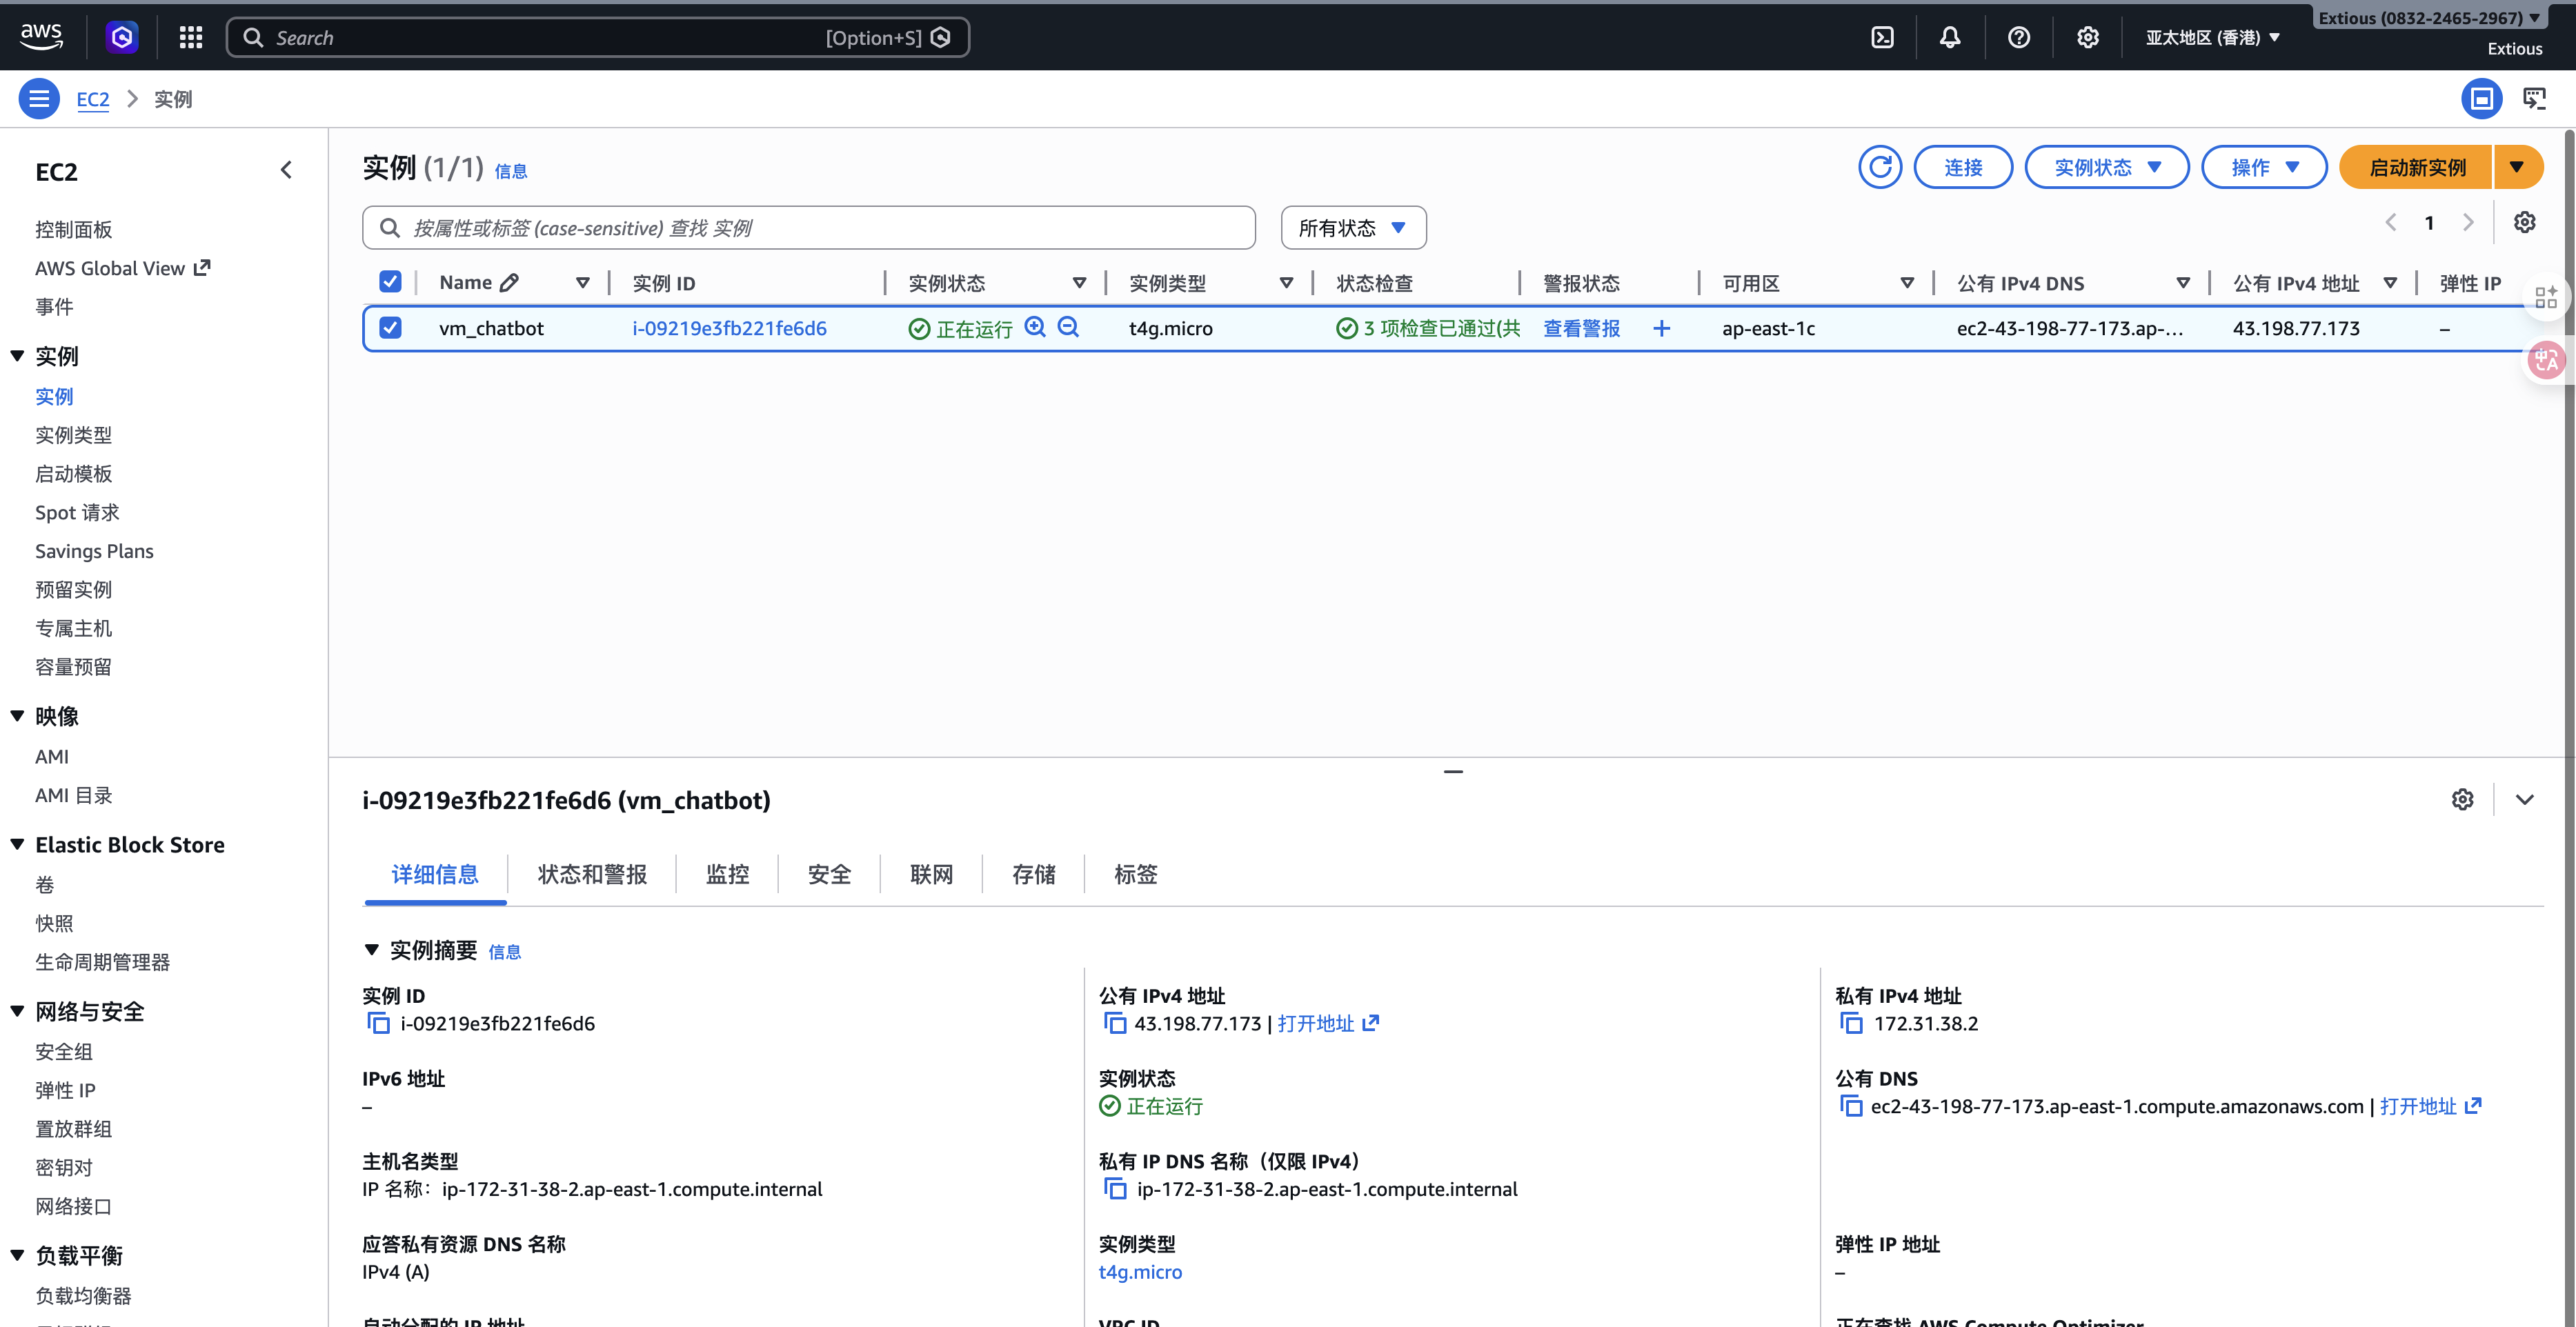
\includegraphics[width=0.95\linewidth]{lab4/instance_information.png}
  \caption{Summary of the EC2 instance \texttt{vm\_chatbot} in the AWS Management Console.}
  \label{fig:instance}
\end{figure}

\section*{2. Chatbot Running on EC2}

After launching the instance, the chatbot program was deployed by uploading \texttt{chatbot.py}, \texttt{ChatGPT\_HKBU.py}, \texttt{config.ini}, and \texttt{requirements.txt} via \texttt{scp}.
A Python 3.12 virtual environment was created on the instance and all dependencies were installed.
The chatbot was then started with \texttt{python chatbot.py} over an SSH session.

Figure~\ref{fig:chat} shows a Telegram conversation with the chatbot running on the EC2 instance.
Figure~\ref{fig:logs} shows the terminal logs from the EC2 SSH session while the chatbot is serving requests.

\begin{figure}[htbp]
  \centering
  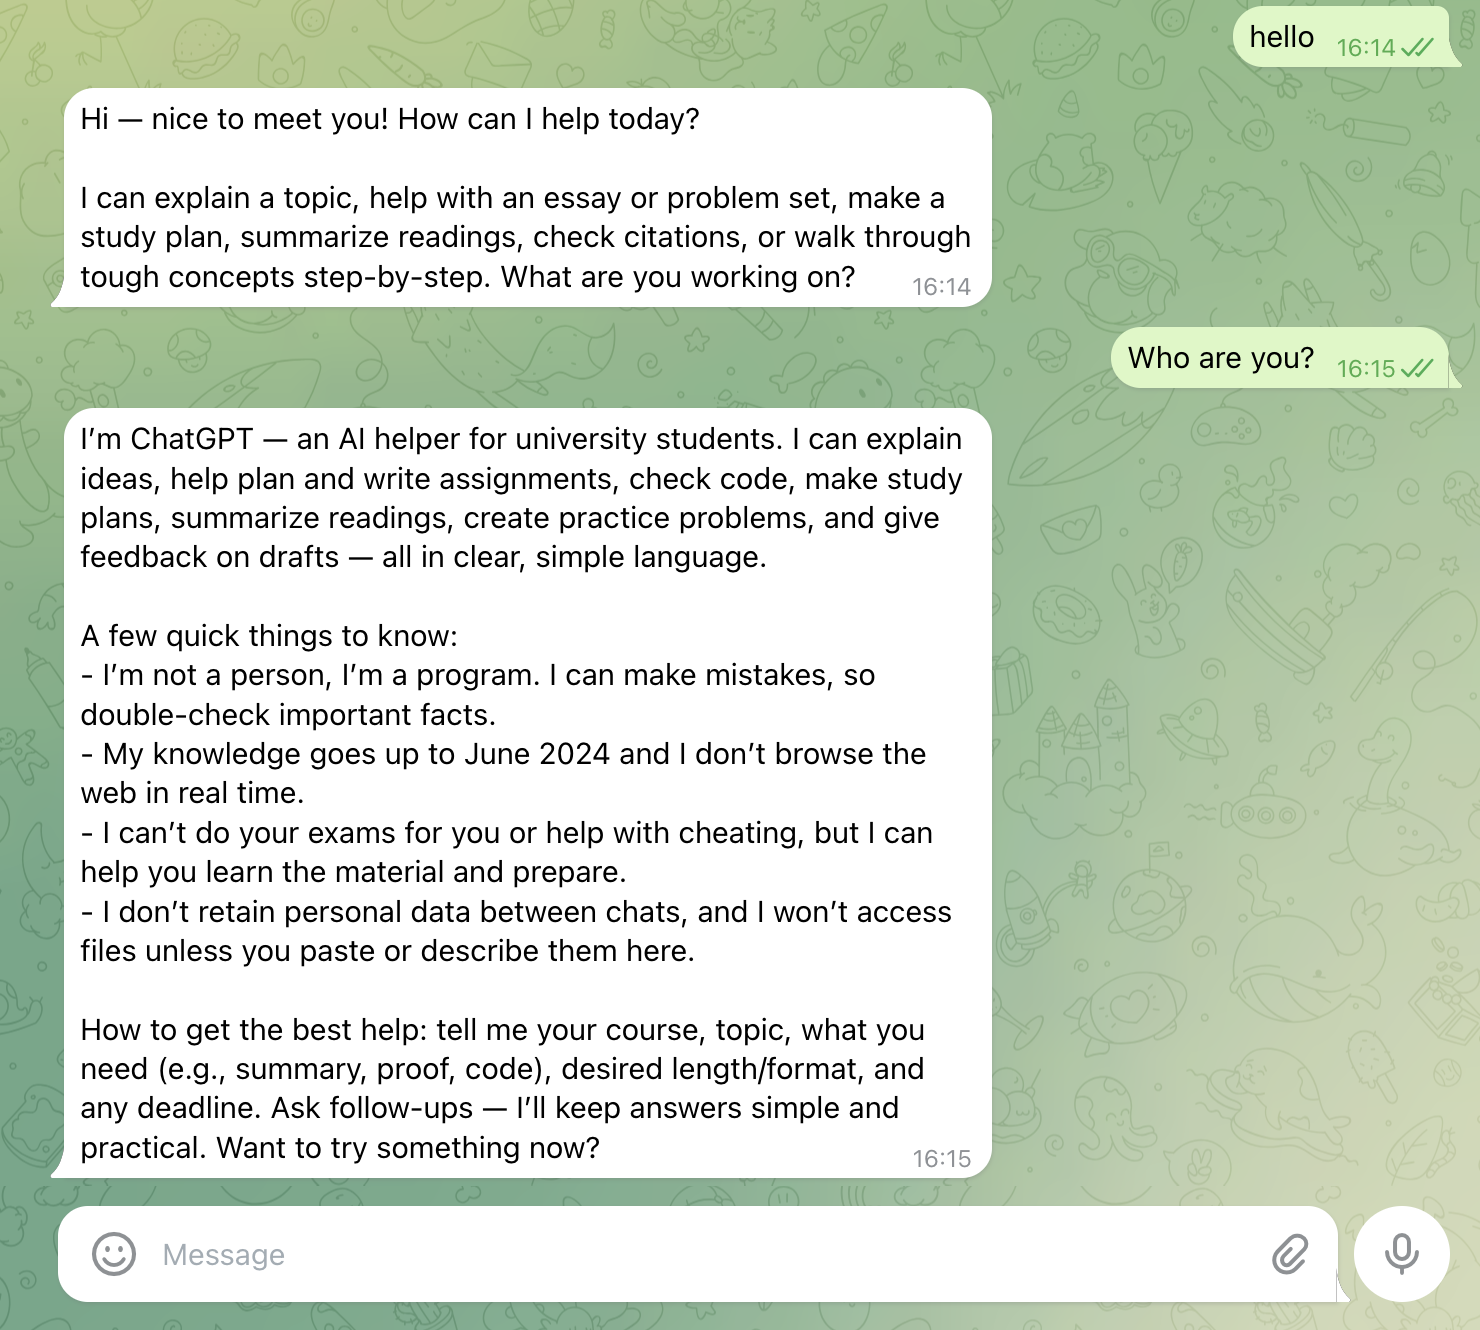
\includegraphics[width=0.6\linewidth]{lab4/chat_example.png}
  \caption{Telegram conversation with the chatbot running on the EC2 instance.}
  \label{fig:chat}
\end{figure}

\begin{figure}[htbp]
  \centering
  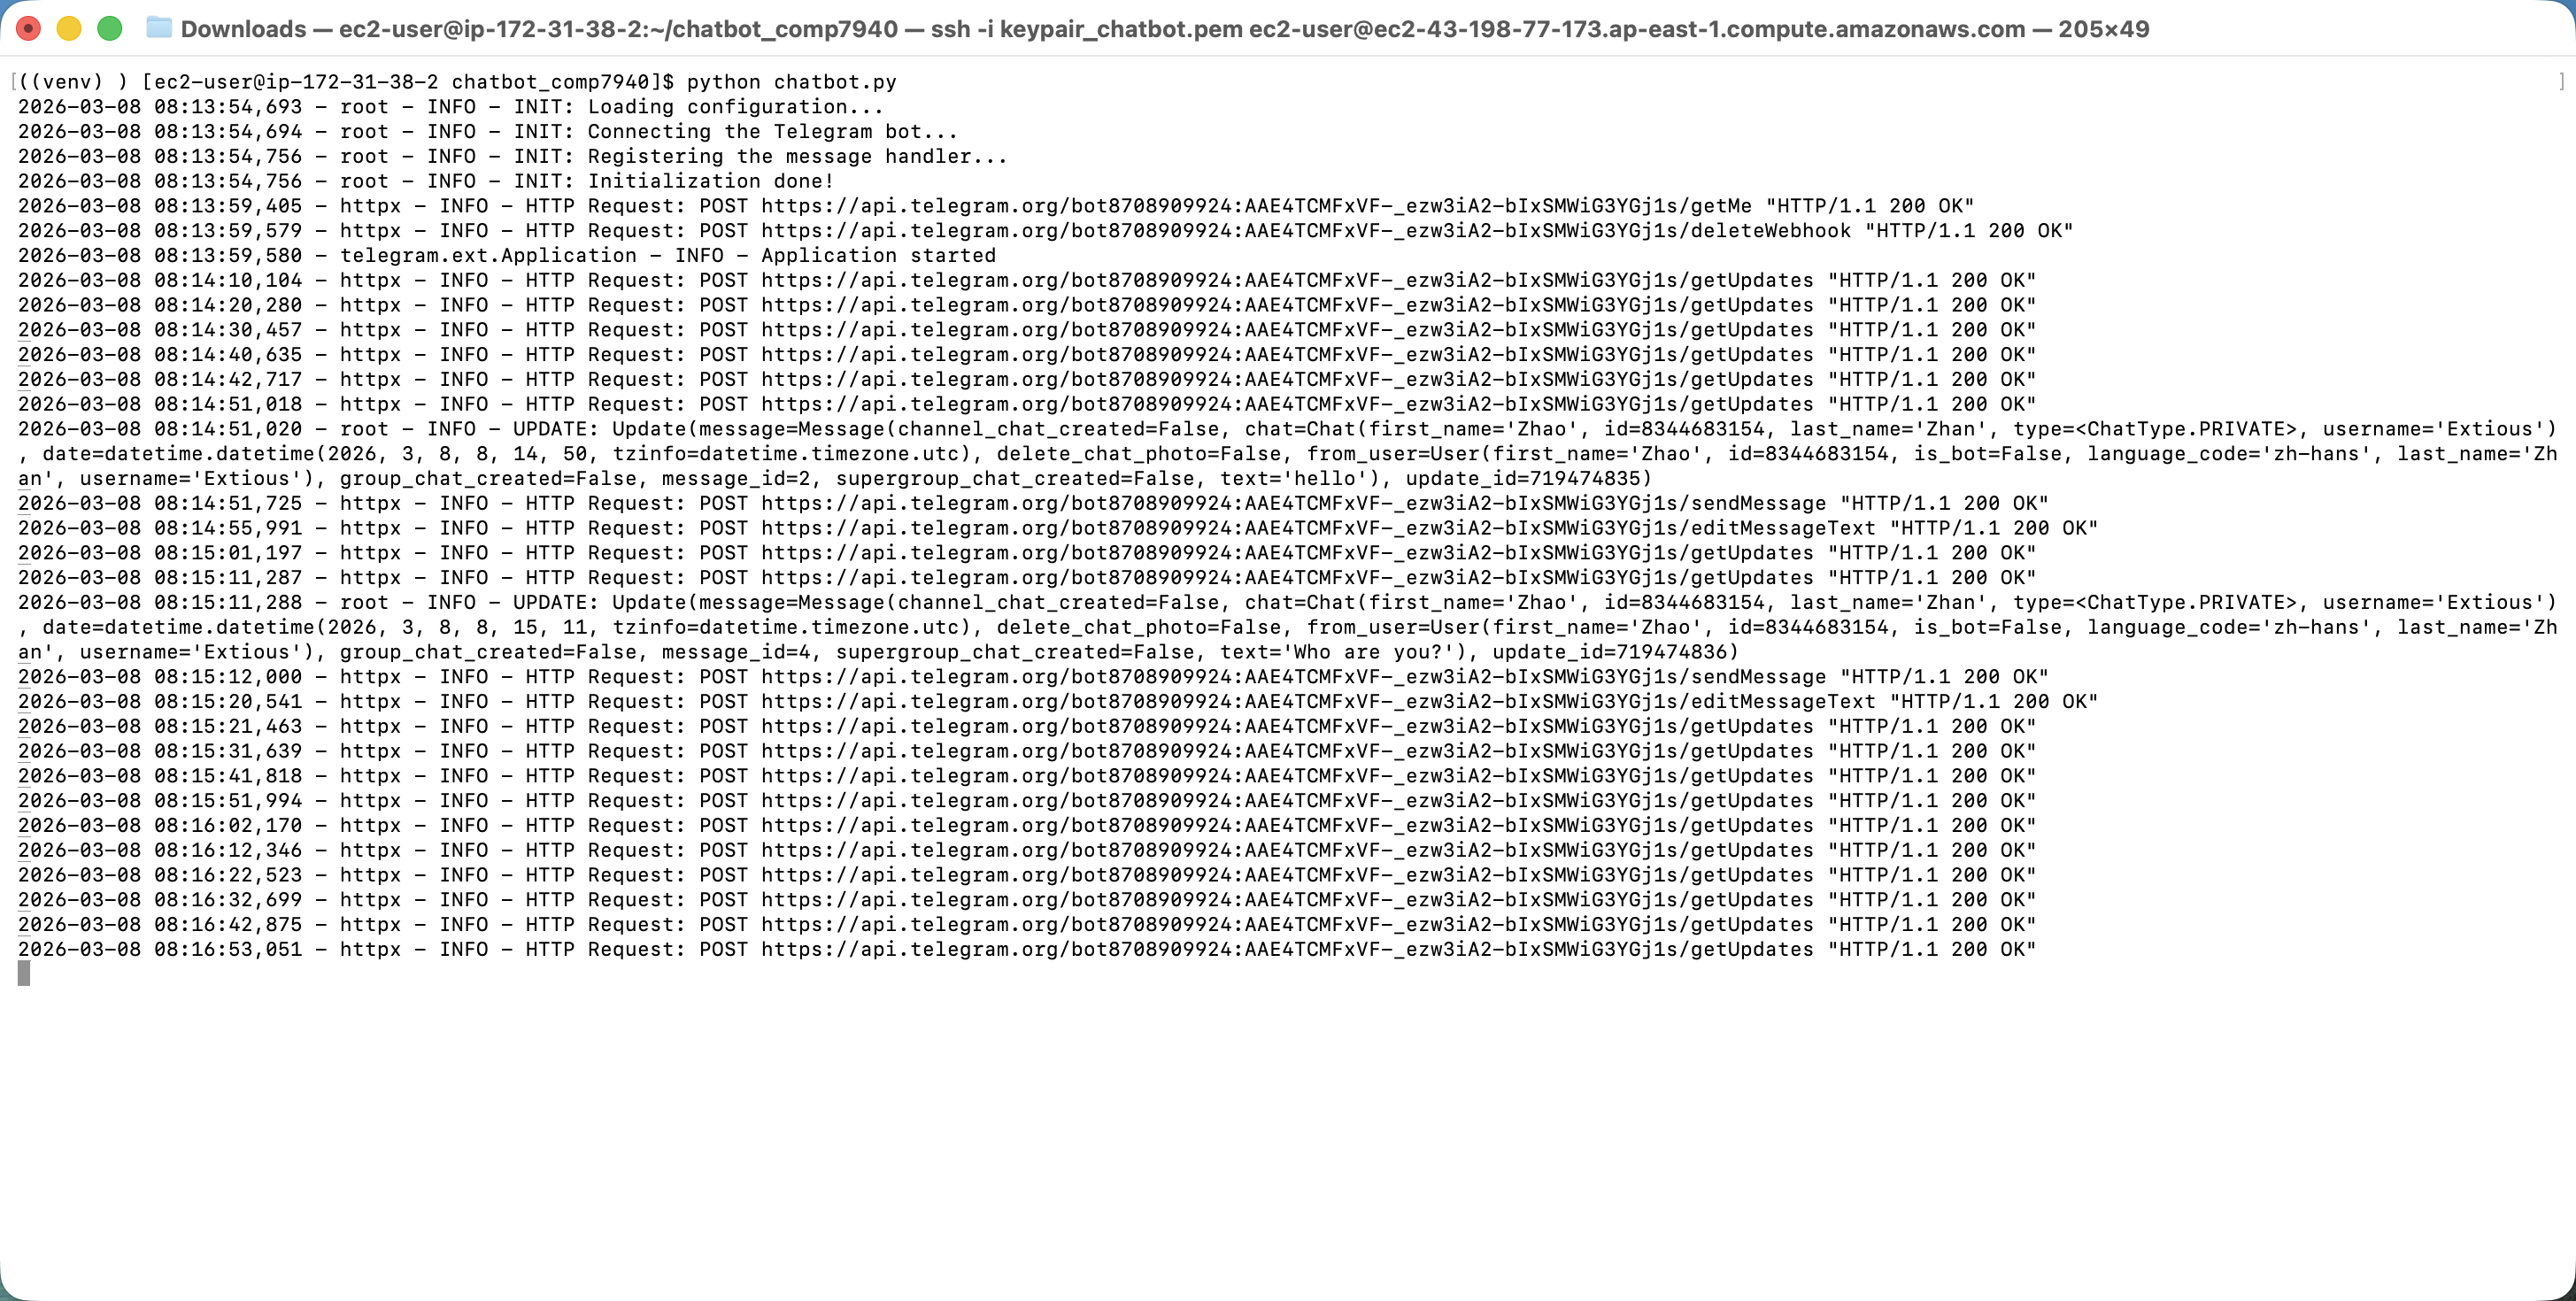
\includegraphics[width=0.95\linewidth]{lab4/terminal_logs.png}
  \caption{Terminal logs from the EC2 instance showing chatbot activity.}
  \label{fig:logs}
\end{figure}

\section*{3. Write-Up Questions}

\subsection*{Q1: Why does Telegram stop responding after the EC2 terminal is closed?}

The chatbot program (\texttt{chatbot.py}) runs as a foreground process inside the SSH session.
It uses long polling~\cite{telegram-bot-api} to continuously fetch new messages from Telegram's servers and send replies.
When the SSH terminal is closed, the operating system sends a \texttt{SIGHUP} (hang-up) signal to all processes associated with that terminal session.
Since the chatbot process is not daemonized or managed by a process supervisor (e.g., \texttt{systemd}, \texttt{nohup}, \texttt{tmux}, or \texttt{screen}), it receives the \texttt{SIGHUP} signal and terminates.
Once the process is terminated, there is no running program to poll for new messages or send responses, so the Telegram bot becomes unresponsive.

To keep the chatbot running after disconnecting, one could use tools such as \texttt{nohup}, \texttt{tmux}, \texttt{screen}, or register the program as a \texttt{systemd} service~\cite{aws-ec2-docs}.

\subsection*{Q2: Why does \texttt{keypair\_chatbot.pem} need to be stored securely and privately?}

The file \texttt{keypair\_chatbot.pem} is the private key of an asymmetric key pair used for SSH authentication to the EC2 instance~\cite{aws-ec2-docs}.
It must be kept secure for the following reasons:

\begin{enumerate}
  \item \textbf{Full access to the instance.}
    Anyone who possesses this private key can establish an SSH connection to the EC2 instance with full shell access, just as if they were the legitimate owner.
    This means they could read, modify, or delete any file on the instance, including source code, configuration files (which may contain API keys and tokens), and system files.

  \item \textbf{No password fallback.}
    By default, EC2 instances created with a key pair do not enable password-based SSH login.
    The \texttt{.pem} file is the \emph{sole} authentication credential.
    If it is compromised, there is no secondary factor to prevent unauthorized access.

  \item \textbf{Irreplaceable by design.}
    AWS does not allow re-downloading the private key after initial creation.
    If the key is lost, the user must create a new key pair and reconfigure instance access.
    If the key is leaked, the attacker retains access until the corresponding public key is explicitly removed from the instance's \texttt{authorized\_keys} file or the instance is terminated.

  \item \textbf{Lateral movement risk.}
    A compromised instance can be used as a pivot point to attack other AWS resources within the same VPC, scan internal networks, or launch further attacks, potentially incurring significant financial and security consequences for the account owner.
\end{enumerate}

Therefore, the private key file should be stored with restrictive file permissions (\texttt{chmod 400}), never shared, never committed to version control, and ideally kept in a secure location such as an encrypted volume or a secrets manager.

\subsection*{Q3: EC2 Instance Summary Screenshot}

The screenshot of the EC2 instance summary is provided in Figure~\ref{fig:instance} (Section~1).

\bibliographystyle{plain}
\bibliography{Lab4-25482351-ZHAOZhan}

\end{document}
